\documentclass[border=8pt]{standalone}
\usepackage{amsmath}
\usepackage{amssymb}
\usepackage{tikz}
\usetikzlibrary{arrows.meta,calc,decorations.pathreplacing,patterns,shapes.geometric,positioning,shadings}

\begin{document}
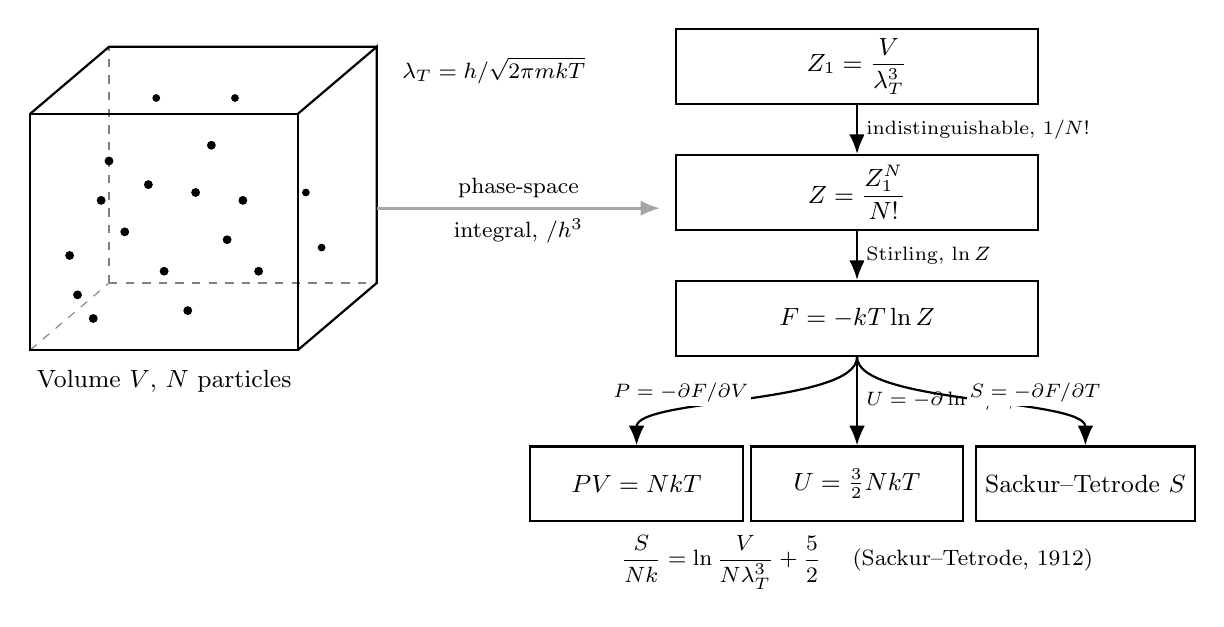
\begin{tikzpicture}[
    >={Latex[length=2.5mm,width=2mm]},
    box/.style={draw, rectangle, minimum width=4.6cm, minimum height=0.95cm, align=center, font=\small, thick, fill=white},
    final/.style={draw, rectangle, minimum width=2.7cm, minimum height=0.95cm, align=center, font=\small, thick, fill=white},
    arrowlbl/.style={font=\scriptsize, midway, fill=white, inner sep=1pt}
]

% ===== LEFT: Ideal gas box (cube) =====
% Cube vertices (isometric-ish)
\coordinate (A) at (0,0);          % front-bottom-left
\coordinate (B) at (3.4,0);        % front-bottom-right
\coordinate (C) at (3.4,3.0);      % front-top-right
\coordinate (D) at (0,3.0);        % front-top-left
\coordinate (E) at (1.0,0.85);     % back-bottom-left
\coordinate (F) at (4.4,0.85);     % back-bottom-right
\coordinate (G) at (4.4,3.85);     % back-top-right
\coordinate (H) at (1.0,3.85);     % back-top-left

% Back edges (dashed, hidden)
\draw[thin, dashed, gray] (E) -- (F);
\draw[thin, dashed, gray] (E) -- (H);
\draw[thin, dashed, gray] (A) -- (E);

% Visible edges (solid)
\draw[thick] (A) -- (B) -- (C) -- (D) -- cycle;       % front face
\draw[thick] (B) -- (F) -- (G) -- (C);                % right + top-back-right
\draw[thick] (D) -- (H) -- (G);                       % top-back-left

% Particles (small filled dots)
\foreach \x/\y in {0.6/0.7, 1.2/1.5, 2.0/0.5, 2.7/1.9, 1.0/2.4, 2.3/2.6, 1.7/1.0, 0.9/1.9, 2.9/1.0, 2.5/1.4, 0.5/1.2, 1.5/2.1, 2.1/2.0, 0.8/0.4} {
    \fill[black] (\x,\y) circle (1.6pt);
}
% A few particles in the depth (between front and back face)
\foreach \x/\y in {1.6/3.2, 2.6/3.2, 3.5/2.0, 3.7/1.3} {
    \fill[black] (\x,\y) circle (1.4pt);
}

% Labels for the box
\node[font=\small] at (1.7,-0.4) {Volume $V$, $N$ particles};
\node[font=\footnotesize, anchor=west] at (4.6,3.55) {$\lambda_T = h/\sqrt{2\pi m kT}$};

% ===== RIGHT: Flow diagram =====
\node[box] (Z1) at (10.5,3.6) {$Z_1 = \dfrac{V}{\lambda_T^{3}}$};
\node[box] (Z)  at (10.5,2.0) {$Z = \dfrac{Z_1^{N}}{N!}$};
\node[box] (F)  at (10.5,0.4) {$F = -kT\ln Z$};

% Final outputs row
\node[final] (P) at (7.7,-1.7)  {$PV = NkT$};
\node[final] (U) at (10.5,-1.7) {$U = \tfrac{3}{2}NkT$};
\node[final] (S) at (13.4,-1.7) {Sackur--Tetrode $S$};

% Arrows on the flow with equations
\draw[->, thick] (Z1) -- (Z)
    node[arrowlbl, right=2pt] {indistinguishable, $1/N!$};
\draw[->, thick] (Z)  -- (F)
    node[arrowlbl, right=2pt] {Stirling, $\ln Z$};

% Three branches from F
\draw[->, thick] (F.south) .. controls +(0,-0.6) and +(0,0.6) .. (P.north)
    node[arrowlbl, above left=-2pt and -2pt] {$P=-\partial F/\partial V$};
\draw[->, thick] (F.south) -- (U.north)
    node[arrowlbl, right=2pt] {$U=-\partial \ln Z/\partial \beta$};
\draw[->, thick] (F.south) .. controls +(0,-0.6) and +(0,0.6) .. (S.north)
    node[arrowlbl, above right=-2pt and -2pt] {$S=-\partial F/\partial T$};

% Bottom note: extensivity + h^3
\node[font=\footnotesize, align=center] at (10.5,-2.7)
    {$\dfrac{S}{Nk} = \ln\dfrac{V}{N\lambda_T^{3}} + \dfrac{5}{2}$ \quad (Sackur--Tetrode, 1912)};

% Connector arrow from box to flow
\draw[->, very thick, gray!70] (4.4,1.8) -- node[font=\footnotesize, above, black]{phase-space} node[font=\footnotesize, below, black]{integral, $/h^3$} (8.0,1.8);

\end{tikzpicture}
\end{document}
